\documentclass[a4paper,12pt]{article}

% don't forget the document class, generally : \documentclass[a4paper,12pt]{article}

\usepackage[utf8]{inputenc}
\usepackage[french]{babel}
\usepackage{graphicx}
\usepackage{gensymb}
\usepackage{amsmath}
\usepackage{float}
\usepackage{scrextend}
\usepackage{caption} 
\usepackage{siunitx}
\usepackage{enumitem}
\usepackage{amsthm}
\usepackage{fancyhdr}
\usepackage{amssymb}
\usepackage{wrapfig}
\usepackage{geometry}
\usepackage{standalone}
\usepackage{import}
\usepackage[usenames, dvipsnames]{color}

 \usepackage{biblatex} % manages bibliography and references
\addbibresource{sample.bib}


\geometry{hmargin=1in, vmargin=1in}

 \newenvironment{absolutelynopagebreak}
 {\par\nobreak\vfil\penalty0\vfilneg
 \vtop\bgroup}
 {\par\xdef\tpd{\the\prevdepth}\egroup
 \prevdepth=\tpd}
 
 \pagestyle{fancy}                        
\fancyhf{}                               
\fancyhf[HL]{Application des maths}                
\fancyhf[HR]{Géométrie euclidienne}             
\fancyhf[FC]{\thepage/\pageref{Lastpage}}
 
\newtheorem{definition}{Définition}[section]
\newtheorem{theorem}{Théorème}
\newtheorem{corollary}{Corollaire}[theorem]
\newtheorem{lemma}[theorem]{Lemme}
\newtheorem*{hyp}{Hypothèse}
\newtheorem*{concl}{Conclusion}
\newtheorem*{remark}{Remarque}

\captionsetup{format=default,labelformat=simple,labelsep=colon,
justification=justified,font={sf,small},labelfont=bf,
textfont=default} 



\begin{document}

\pagebreak
\subsection{Triangles isocèles}
\begin{theorem}
Un triangle est isocèle si et seulement si les angles opposés aux côtés isométriques sont isométriques.
\end{theorem}

\begin{proof}
La démonstration de ce théorème se déroule en deux parties:
\begin{itemize}
    \item La première partie doit démontrer qu'un triangle avec deux côtés isométriques est isocèle
    \item La deuxième partie doit démontrer qu'un triangle avec deux angles isométriques est isocèle
    \end{itemize}

    \begin{enumerate}
        \item Nous considérons le triangle $ABC$.
        \begin{figure}[H]
        \centering
        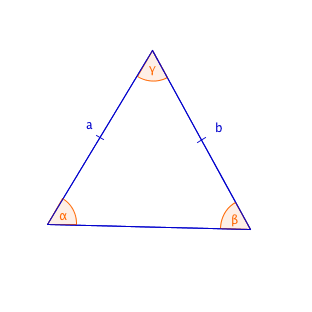
\includegraphics[scale=0.7]{theorems/isocel/iso1.png}
    \end{figure}
    
    
    \begin{hyp}
    $a\equiv b$
    \end{hyp}
    \begin{concl}
    $\alpha \equiv \beta$
    \end{concl}
    En faisant la bissectrice B de l'angle $\gamma$, nous obtenons deux triangles (1 et 2) qui ont un angle isométrique ($\gamma_1 \equiv \gamma_2$) compris entre deux côtés isométriques ($a\equiv b$, B). Donc nous savons que les triangles 1 et 2 sont isométriques, grâce au premier cas d'isométrie des triangles. Par conséquant, $\alpha \equiv \beta$ et le triangle $ABC$ est isocèle.
    
    
    \begin{figure}[H]
        \centering
        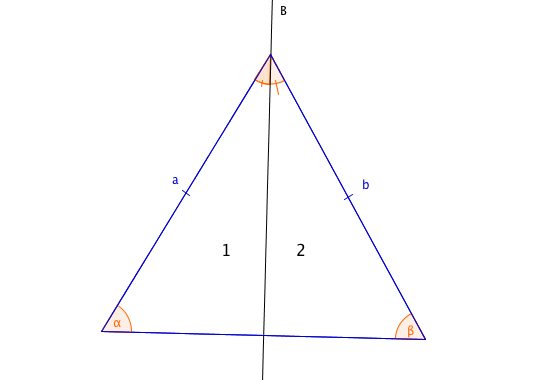
\includegraphics[scale=0.45]{theorems/isocel/iso2.png}
    \end{figure}
    
    
    
    
    \item Nous considérons le triangle $ABC$.
    \begin{figure}[H]
            \centering
            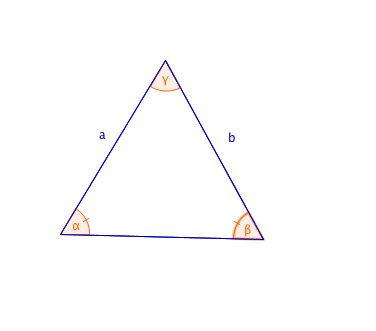
\includegraphics[scale=0.7]{theorems/isocel/iso3.png}
    \end{figure}

    \begin{hyp}
     $\alpha \equiv \beta$
    \end{hyp}
    \begin{concl}
     $a\equiv b$
    \end{concl}
    Nous tirons la hauteur h partant de $\gamma$ et obtenons deux triangles 1 et 2. Ces deux triangles ont deux angles ($\alpha \equiv \beta$, les angles droits) et un côté (h) isométriques, donc ils sont isométriques (corollaire du deuxième cas d'isométrie des triangles). Par conséquent $a\equiv b$ et le triangle $ABC$ est isocèle.
    
    \begin{figure}[H]
        \centering
        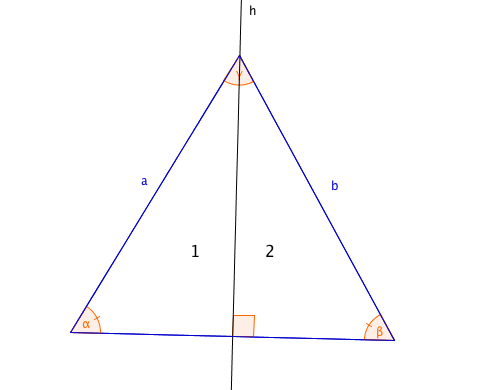
\includegraphics[scale=0.45]{theorems/isocel/iso4.png}
    \end{figure}
    
\end{enumerate}
\end{proof}

\end{document}
